\section{Poisson distribution}

\begin{table}[H]
    \hfill
    \begin{minipage}{0.45\linewidth}
        \begin{figure}[H]
            \centering
            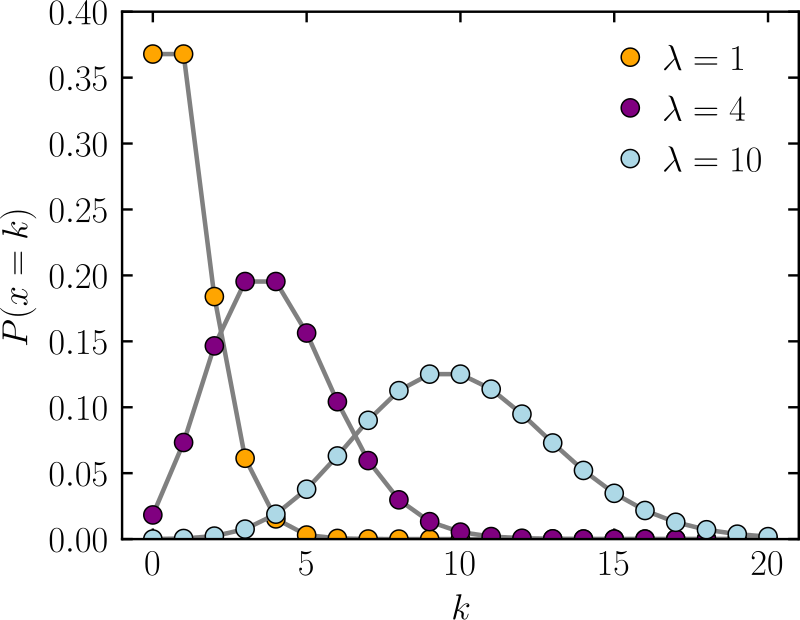
\includegraphics[
                width=\linewidth,
                height=5cm,
                keepaspectratio,
            ]{images/distributions/Poisson_pmf.svg.png}
            \caption{Poisson distribution: PDF \cite{wiki/Poisson_distribution}}
        \end{figure}
    \end{minipage}
    \hfill
    \begin{minipage}{0.45\linewidth}
        \begin{figure}[H]
            \centering
            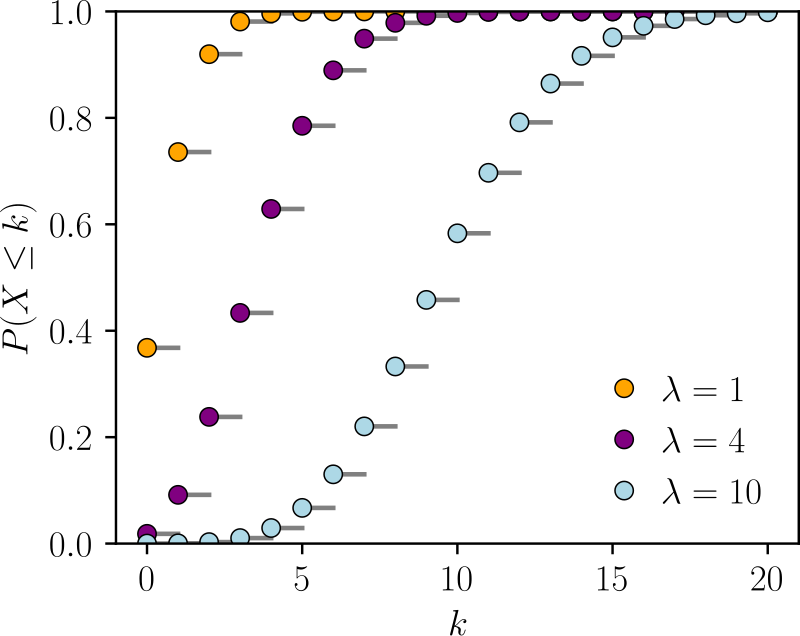
\includegraphics[
                width=\linewidth,
                height=5cm,
                keepaspectratio,
            ]{images/distributions/Poisson_cdf.svg.png}
            \caption{Poisson distribution: CDF \cite{wiki/Poisson_distribution}}
        \end{figure}
    \end{minipage}
    \hfill
\end{table}







\subsection{Summary}

\begin{enumerate}
    \item \textbf{Notation}:
    $
         {\displaystyle \operatorname {Pois} (\lambda )}
    $
    \hfill \cite{wiki/Poisson_distribution}

    \item \textbf{Parameters}:
    ${\displaystyle \lambda \in (0,\infty )}$ (rate)
    \hfill \cite{wiki/Poisson_distribution}

    \item \textbf{Support}:
    ${\displaystyle k\in \mathbb {N} _{0}}$ (Natural numbers starting from $0$)
    \hfill \cite{wiki/Poisson_distribution}

    \item \textbf{PMF}:
    $
         {\displaystyle {\dfrac {\lambda ^{k}e^{-\lambda }}{k!}}}
    $
    \hfill \cite{wiki/Poisson_distribution}

    \item \textbf{CDF}:
    ${\displaystyle {\dfrac {\Gamma (\lfloor k+1\rfloor ,\lambda )}{\lfloor k\rfloor !}},}$ or
    ${\displaystyle e^{-\lambda }\sum _{j=0}^{\lfloor k\rfloor }{\dfrac {\lambda ^{j}}{j!}},}$ or
    ${\displaystyle Q(\lfloor k+1\rfloor ,\lambda )}$
    (for ${\displaystyle k\geq 0,}$ where ${\displaystyle \Gamma (x,y)}$ is the upper incomplete gamma function, ${\displaystyle \lfloor k\rfloor }$ is the floor function, and ${\displaystyle Q}$ is the regularized gamma function)
    \hfill \cite{wiki/Poisson_distribution}

    \item \textbf{Mean}:
    $
         {\displaystyle \lambda }
    $
    \hfill \cite{wiki/Poisson_distribution}

    \item \textbf{Median}:
    $
         {\displaystyle \approx \left\lfloor \lambda +{\dfrac {1}{3}}-{\dfrac {1}{50\lambda }}\right\rfloor }
    $
    \hfill \cite{wiki/Poisson_distribution}

    \item \textbf{Mode}:
    $
         {\displaystyle \left\lceil \lambda \right\rceil -1,\left\lfloor \lambda \right\rfloor }
    $
    \hfill \cite{wiki/Poisson_distribution}

    \item \textbf{Variance}:
    $
         {\displaystyle \lambda }
    $
    \hfill \cite{wiki/Poisson_distribution}

    % \item \textbf{Median absolute deviation (MAD)}:
    % $
    % $
    % \hfill \cite{wiki/Poisson_distribution}

    \item \textbf{Skewness}:
    $
         {\displaystyle {\dfrac {1}{\sqrt {\lambda }}}}
    $
    \hfill \cite{wiki/Poisson_distribution}

    \item \textbf{Excess kurtosis}:
    $
         {\displaystyle {\dfrac {1}{\lambda }}}
    $
    \hfill \cite{wiki/Poisson_distribution}

    \item \textbf{Entropy}:
    ${\displaystyle \lambda {\Bigl [}1-\log(\lambda ){\Bigr ]}+e^{-\lambda }\sum _{k=0}^{\infty }{\dfrac {\lambda ^{k}\log(k!)}{k!}}}$
    or for large ${\displaystyle \lambda }$
    ${\displaystyle {\begin{aligned}\approx {\dfrac {1}{2}}\log \left(2\pi e\lambda \right)-{\dfrac {1}{12\lambda }}-{\dfrac {1}{24\lambda ^{2}}}\\-{\dfrac {19}{360\lambda ^{3}}}+{\mathcal {O}}\left({\dfrac {1}{\lambda ^{4}}}\right)\end{aligned}}}$
    \hfill \cite{wiki/Poisson_distribution}

    \item \textbf{Moment-generating function (MGF)}:
    $
         {\displaystyle \exp \left[\lambda \left(e^{t}-1\right)\right]}
    $
    \hfill \cite{wiki/Poisson_distribution}

    \item \textbf{Characteristic function (CF)}:
    $
         {\displaystyle \exp \left[\lambda \left(e^{it}-1\right)\right]}
    $
    \hfill \cite{wiki/Poisson_distribution}

    \item \textbf{Probability-generating function (PGF)}:
    $
         {\displaystyle \exp \left[\lambda \left(z-1\right)\right]}
    $
    \hfill \cite{wiki/Poisson_distribution}

    \item \textbf{Fisher information}:
    $
         {\displaystyle {\dfrac {1}{\lambda }}}
    $
    \hfill \cite{wiki/Poisson_distribution}
\end{enumerate}




\subsection{Standard Error of MLE}

\begin{enumerate}
    \item let $X_1 , X_2, \cdots , X_n$ be i.i.d. Poisson $\mathcal{P}(\lambda)$ distributed.
    \hfill \cite{statistics/book/Statistics-for-Data-Scientists/Maurits-Kaptein}

    \item population mean $\mu ( f ) = \lambda $ and the population variance $\sigma 2( f ) = \lambda $.
    \hfill \cite{statistics/book/Statistics-for-Data-Scientists/Maurits-Kaptein}

    \item The maximum likelihood estimator for $\theta = \lambda$ , which is also the moment estimator, is given by the sample average $\hat{\lambda} = \bar{X}$.
    \hfill \cite{statistics/book/Statistics-for-Data-Scientists/Maurits-Kaptein}

    \item  the log likelihood is $\ell _\theta = \dsum^n _{i=1}[X_i \log(\lambda ) - \log(X_i !) - \lambda ]$.
    \hfill \cite{statistics/book/Statistics-for-Data-Scientists/Maurits-Kaptein}

    \item Equating the derivative with respect to $\lambda $ to zero results into $\dsum \dParenBrac{\dfrac{X_i}{\lambda} - 1} = 0$.
    Solving this for $\lambda $ gives $\hat{\lambda} = \bar{X}$.
    \hfill \cite{statistics/book/Statistics-for-Data-Scientists/Maurits-Kaptein}

    \item As the distribution of $\dfrac{\sqrt{n}( \bar{X} - \mu ( f ))}{\sigma ( f )}$ converges to a standard normal distribution, $\sqrt{n}( \bar{X} - \lambda )$ converges to $\mathcal{N} (0, \lambda )$
    \hfill \cite{statistics/book/Statistics-for-Data-Scientists/Maurits-Kaptein}

    \item he Fisher information for the Poisson distribution is given by $I (\lambda ) = \mbbE\dSquareBrac{\dParenBrac{\dfrac{X}{\lambda} - 1}2}=  \mbbE\dSquareBrac{\dParenBrac{\dfrac{X - \lambda}{\lambda}}^2} = \dfrac{1}{\lambda} $ .
    \hfill \cite{statistics/book/Statistics-for-Data-Scientists/Maurits-Kaptein}

    \item Thus, the asymptotic variance of the MLE is given by $I ^{-1}(\lambda ) = \lambda $ and the standard error of $\bar{X}$ is equal to $\sqrt{\dfrac{\lambda}{n}}$.
    \hfill \cite{statistics/book/Statistics-for-Data-Scientists/Maurits-Kaptein}
\end{enumerate}




\subsection{Sums of Random Variables}

\begin{enumerate}
    \item Let $U$, $V$, and $W$ be three independent random variables and define $X = W + U$ and $Y = W + V$.
    When $U \sim \mathcal{P}(\lambda _U )$, $V \sim \mathcal{P}(\lambda _V )$, and $W \sim \mathcal{P}(\lambda _W )$, it can be shown that $X$ is Poisson distributed with parameter $\lambda _W + \lambda _U$ and $Y$ is Poisson distributed with parameter $\lambda _W + \lambda _V$.
    \hfill \cite{statistics/book/Statistics-for-Data-Scientists/Maurits-Kaptein}

    \item PDF:
    $
        f _{X Y} (x, y)
        = \exp(-[\lambda _U + \lambda _V + \lambda _W ])\ \dfrac{\lambda ^x_U \lambda ^y_V} {x!\ y!}
        \ \dsum^{\min(x,y)} _{k=0} \dfrac{x!\ y! }{(x - k)!\ (y - k)!\ k!} \dParenBrac{\dfrac{\lambda _W }{\lambda _U \lambda _V} }^k
    $
    \hfill \cite{statistics/book/Statistics-for-Data-Scientists/Maurits-Kaptein}
\end{enumerate}








